\chapter{Introduction}\label{sec:introduction}

While the success of deep learning models has been rapid, the theoretical
justification for most game-changing ideas as well as the general principles of
deep learning has not kept pace (for more information, see \cite{arora2018}).
This means that for many successful techniques, we have no clear understanding
why they work so well in practice.

This explanatory gap is also a reason why developing deep learning applications
is considered more of an art than a science. In contrast to traditional
programming, which builds on decades of research and development in electrical
engineering, logic, mathematics and theoretical computer science, there's rarely
one definitive way to solve a certain problem in deep learning.  Additionally,
the quality of debugging tools available to a programmer on every level of
abstraction far exceeds what we currently have for differentiable programming.
Simple questions like ``Does my model learn what I want it to learn?'' are not
answerable at this point.  We can thus identify a need to supply more useful
tooling for deep learning researchers and practitioners.  A standard approach to
choosing a parametrisation remains trial-and-error, or only somewhat more
sophisticated ways to run and test.  The computational cost of training large
models prohibits quick experimentation and often translates into monetary costs
as well.  Identifying dead ends early or points in training at which to tweak
certain parameters could thus provide large savings in time and money, besides
enabling a more thorough understanding of what is going on inside the pile of
linear algebra that is a deep learning model.

This thesis addresses the above in two ways: A software library aiding in deep
learning debugging and experimentation is designed, implemented and documented. The same
library is then used to investigate experimentally whether unexplored
metrics can be devised for optimising parameters of the training process while it is running.

This thesis is concerned with \emph{deep} neural networks, meaning
architectures consisting of many layers. Typically, the number of units
in such a model and thus the number of tunable parameters
(\(n_{weights\_per\_neuron} \times n_{neurons}\)) exceeds the number of
training examples. Training such large networks thus involves iterating
over the dataset many times which incurs a high computational cost due
to the massive number of matrix operations involved. Speeding up the
training is thus one of the primary endeavours in deep learning
research. An overview of the workings of a neural network is given in
\cref{sec:anns}.

\hypertarget{sec:anns}{%
\section{Artificial Neural Networks}\label{sec:anns}}

For the reader's benefit, a brief introduction to artificial neural networks is
presented here, which may safely be skipped or replaced by other resources.

\subsection*{A Brief History of Neural Networks}%

The artificial neural network is a class of machine learning model which can be
used for prediction tasks like regression and classification, as well as for
generation and enhancement of data.  At
the core, neural models are simply conceptualised as an arrangement of units
which receive numerical inputs, compute a weighted sum and thus produce an output
activation. The ideas date back at least to Hebbian learning (a single neuron)
in the 1940s, and were developed into the Perceptron model by
\citet{Rosenblatt58theperceptron}. With the introduction of the backpropagation
algorithm \citep{werbos1975beyond} and increasing availability of computing
power, this began to change, but more easily trainable models like Support
Vector machines eclipsed neural nets for most applications.  Architectural
advances, such as the convolutional neural networks in the late 1980s
\citep{LeCun:1989:BAH:1351079.1351090} and the advent of GPU-accelerated neural
network implementations (pioneered in \cite{Ciresan11flexible})---as well as
subsequently, gpu-accelerated linear algebra libraries with automatic
differentiation---finally made neural networks the workhorse for many AI
applications today.

\subsection*{A Brief Primer on Neural Networks}%

A neural network consists of at least one input layer, \(0-n\)
intermediate layers and at least one output layer. Data is processed in
numerical form by multiplying it with the input layer's weights, mapping
each product with the input layer's activation function and then
propagating the resulting activations through subsequent layers in the
same fashion. \Cref{fig:neuralnet} gives a graphical representation of a
multi-layer feedforward network, the simplest form of neural network.
Mathematically, such a model corresponds to a set of weight matrices
$\mathcal{W} = \{W_i \mid W \in \mathbf{R}^{n_{i-1} \times n_i}\}$ where $n_i$
is the number of units in layer $i$. Each layer can have an associated bias
vector that is added to the output. The computation performed by layer $i$ on
the previous layer's output is
thus
\begin{align}
    f_i(\mathbf{x}) = W_i \mathbf{x} + b_i
\end{align}

If only matrix multiplication and vector addition was used, a multi-layer network would be no more
powerful than a single-layer one as the composition of many affine
transformations can be expressed by a single one. Therefore, a nonlinear
\emph{activation function} is applied component-wise to each layer's output. The
nonlinearity is crucial to deeper networks superior capabilities. Many
activation functions have been proposed, for instance the hyperbolic tangent,
the sigmoid or the rectified linear unit, the latter in many variations.
\Cref{fig:activation_functions} shows plots for these functions.

\pgfmathdeclarefunction{sigmoid}{0}{%
    \pgfmathparse{1/(1+exp(-x))}%
}
\pgfmathdeclarefunction{relu}{0}{%
    \pgfmathparse{((x<0) * 0 + (x>=0) * x)}%
}
\begin{figure}
    \centering
    \begin{tikzpicture}[
            declare function={
                func(\x) = (\x<0) * (0)  +  (\x>=0) * (\x);
            }
        ]
        \begin{groupplot}[group style={group size= 3 by 1}, ymin=-1, ymax=2, xmin=-5,
            xmax=5, width=.32\linewidth, tick label style={font=\tiny}]
            \nextgroupplot[title=sigmoid]
            \addplot[verydarkblue] {sigmoid};
            \nextgroupplot[title=tanh]
            \addplot[reddish] {tanh(x)};
            \nextgroupplot[title=ReLU]
            \addplot[yellowish] {func(x)};
        \end{groupplot}
    \end{tikzpicture}
    \caption{Shapes of different activation functions}
    \label{fig:activation_functions}
\end{figure}

\begin{figure}
    \hypertarget{fig:neuralnet}{%
        \centering
        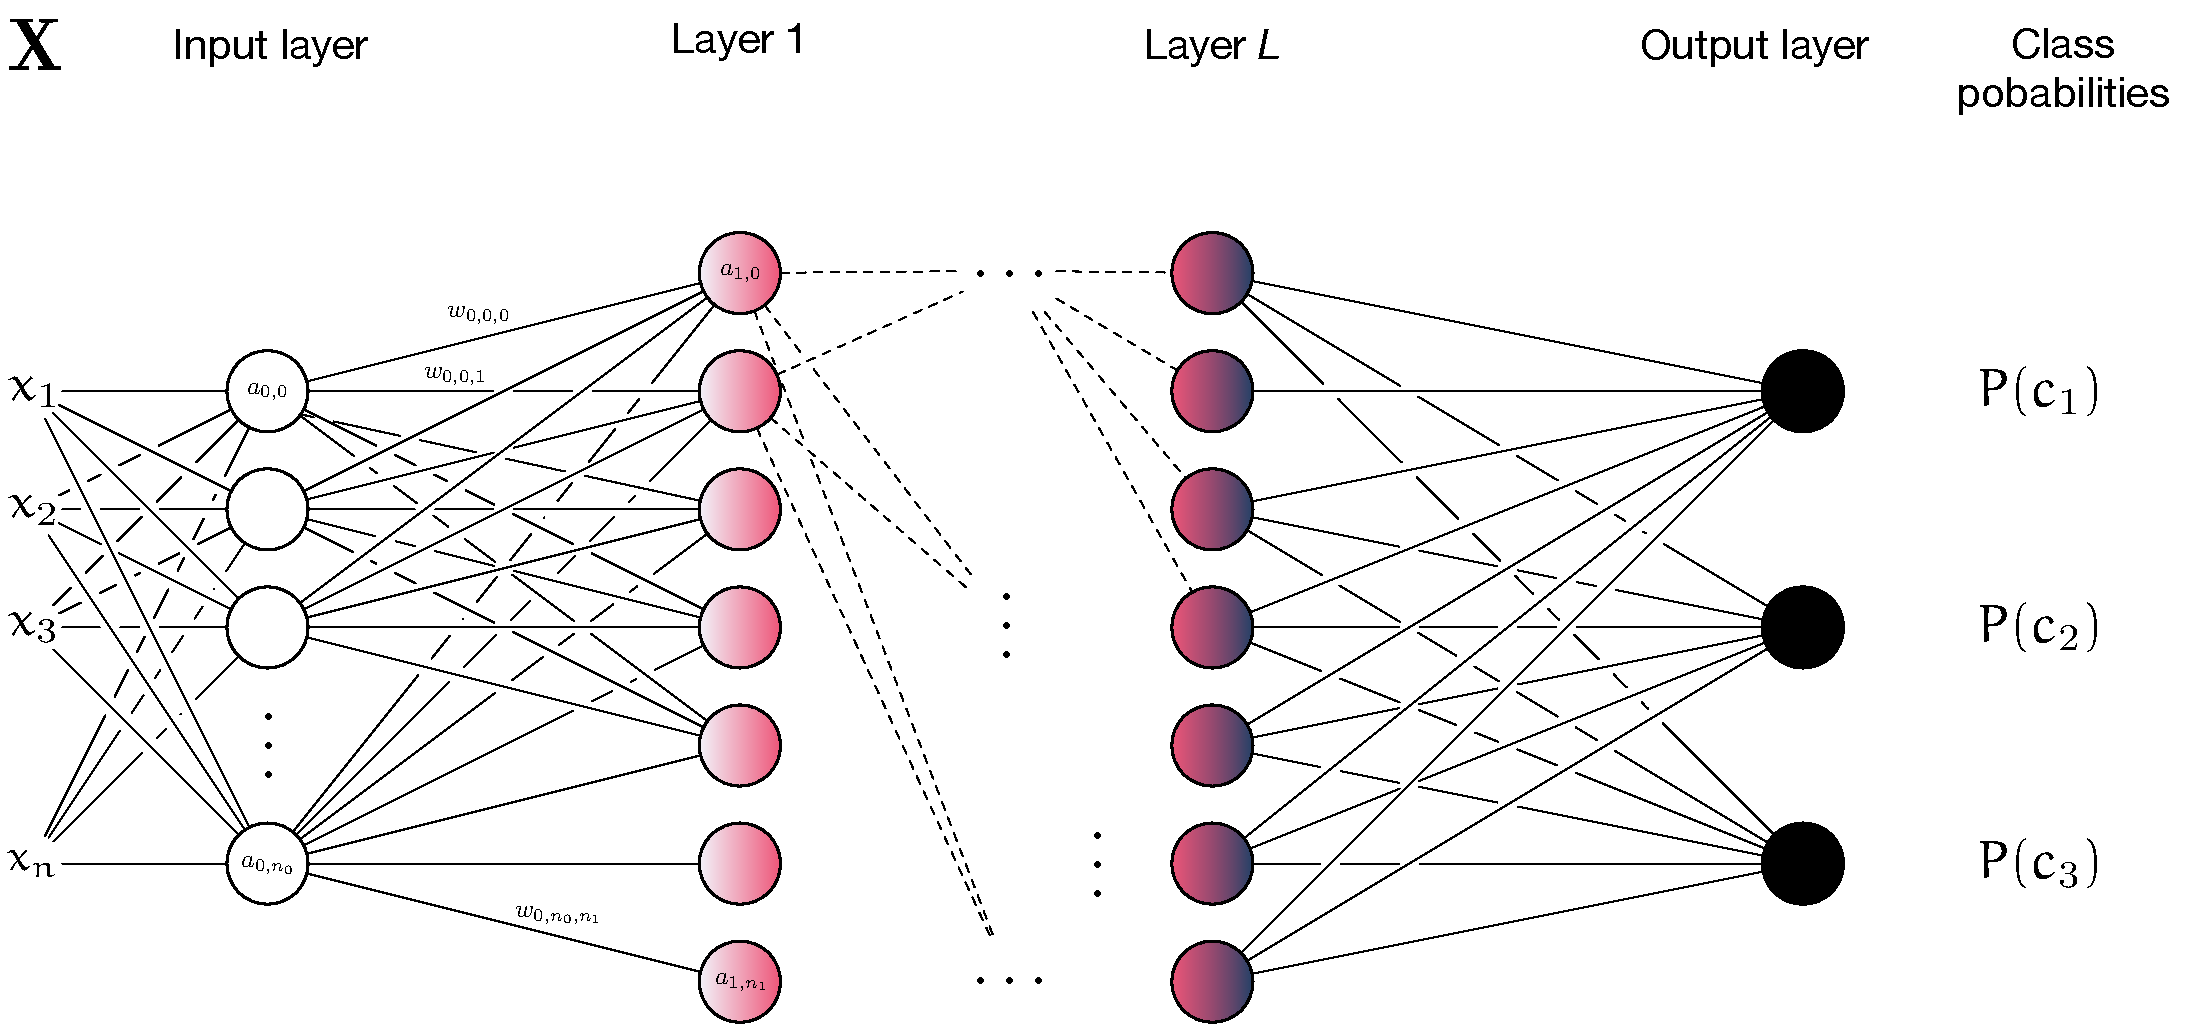
\includegraphics[max width=\textwidth]{gfx/diagrams/neural_network/neural_net.pdf}
        \caption[Schema of a multi-layer neural network]{Schema of a multi-layer neural network. \(\mathbf{x}_i\) are
            the input values, \(a_{l_n,i}\) the \(i\)-th activation in layer \(l_n\)
            and \(w_{l_n,i,j}\) the weight between the \(i\)-th unit in layer
        \(l_n\) and the \(j\)-th unit in layer \(l_{n+1}\)}\label{fig:neuralnet}
    }
\end{figure}

Training a neural network simply involves a loss function measuring the distance
of the networks output to the desired output and differentiating it with respect
to the model parameters. The backpropagation algorithm provides an efficient way
of computing all the partial derivatives of the loss with respect to each
parameter (network weight). Parameters are usually updated with some form of the
gradient descent optimisation algorithm. An introduction to the mathematics of
deep neural networks is deferred to
\cref{sec:review_stochastic_gradient_descent}.

\hypertarget{sec:thesis-goals}{%
\section{Goals of this Thesis}\label{sec:thesis-goals}}

The objective of this work is twofold:

\begin{enumerate}
    \item
        Create a software library that enables easy and reusable
        implementation of training metrics and abstracts away the concrete model
        architecture
    \item
        Perform experiments on common datasets to investigate whether common
        problems in neural network training can be detected on-line by the use of
        appropriate metrics. In other words, the library shall be used to
        verify or falsify that training dynamics can be analyzed during
        training. Issues which could be investigated include, but are
        not limited to
        \begin{itemize}
            \item
                inappropriate learning rate
            \item
                layer/model saturation
            \item
                bad initialisations
            \item
                inappropriate network architecture
            \item
                bad generalisation/overfitting
            \item
                susceptibility to adversarial attacks
        \end{itemize}
\end{enumerate}

\hypertarget{sec:motivation}{%
\section{Motivation}\label{sec:motivation}}

In contrast to classical machine learning models, training deep neural networks
requires navigating a huge parameter space. While most non-neural regression or
classification algorithms only require specification of a parameter set up-front
and often no more than a few, some parameters can (and should) be varied over
training time for neural networks. Looking at the popular scikit-learn library \citep{scikit-learn},
it can be seen that traditional methods such as SVMs, Gaussian Processes,
Decision Trees or Gradient Boosting typically require less than $10$
hyperparameters\footnote{A look through
\href{http://scikit-learn.org/stable/supervised_learning.html\#supervised-learning}{scikit-learn}s
selection of regressors and classifiers shows most classes require between 5 and
10 parameters.}.

In neural networks the parameter space can have arbitrarily many dimensions when
factoring in the fact that some parameters can change over time, such as

\begin{itemize}
    \item
        learning rate (can vary according to some schedule)
    \item
        batch size\footnote{It is not usual to change the batch size during
            training, but it can have an effect similar annealing the learning
        rate (see \cite{DBLP:journals/corr/abs-1711-00489})}
    \item
        trainability of layers (not all layers need to be trained throughout the
        entire training)
\end{itemize}

Other parameters that need to be set initially are

\begin{itemize}
    \item
        network architecture (how many layers, how many units per layer,
        what kind of layers)
    \item
        nonlinearity function for each layer
    \item
        loss function
    \item
        optimisation algorithm
    \item
        initial learning rate
    \item
        momentum of the weight updates
    \item
        weight decay
    \item
        regularisation methods for the weights
\end{itemize}

This makes finding an optimal training regimen very hard, particularly since
training deep neural networks for realistic problems can take much longer than
traditional methods, meaning cross-validating different models can be
prohibitively expensive. It is therefore desirable to notice dead ends early
during training, or be able to tweak parameters in such a way as to maximise
convergence speed.

This thesis work is motivated by the scarcity of useful tools to debug and
monitor deep learning training. \citet{arpteg2018software} discuss several
challenges arising in the context of engineering larger-scale machine learning
software and note that a lack of useful debugging tools can lead to a lot of
wasted time and money in diagnosing problematic behaviour of a neural network.

Without years of training and a lot of
mathematical intuition and expertise, it is often very hard to figure out why a
network is not learning or how to ensure timely convergence.  And even with this
expertise, visualisations or metrics need to be implemented over and over again
because common tools do not abstract from the concrete model architecture.
Providing easy-to-use tooling and live insights also has the side-effect of
democratising access to machine learning software. Ideally, the metrics created
with the help of this work would enable non-experts to better understand their
models and reduce the dependence on rare machine learning expertise. While this
goal will likely not be achieved by this work alone, steps in the general
direction are needed for disseminating AI advances throughout the industry, and
counteract the tendency of large companies to reap the majority of the benefits
brought about by deep learning.

There exist some monitoring tools (see \cref{sec:existing-apps}), but they
are mostly low-level tools which provide visualisation primitives (drawing and
interacting with graphs). They may enable visualisation of certain network
metrics on top of the primitives, but there is no native support for a concept
such as \emph{Maximum singular value of the weight matrix} which can be simply
applied automatically to all layers.

In contrast, the library developed in this work is geared towards modularising
introspection metrics in such a way that they are usable for any kind of model,
without modifications to the model code. The secondary purpose of the library is
the enablement to quickly iterate on hypothesised metrics extracted from the
training in order to diagnose problems such as those outlined in
\cref{sec:thesis-goals}. Most deep learning research involves experiments on a
variety of architectures, datasets, and hyperparameter sets in order to validate
an idea. All of these experiments must be implemented, which can easily lead to
haphazard duplication of code for all the different settings, or creation of
ad-hoc libraries that are only used in this specific work. Thus, a lot of effort
is wasted due to the lack of more general tools and the fact that code produced
for research often is not made public, or would require significant effort to
generalise to other problems.

As such, the library shall not only be useful to end users who will make use of
established metrics and thus save time in their model training, but also to
researchers and the author of this thesis in evaluating hypotheses about
training metrics.

In summary, this library is supposed to be both a developer tool, reducing
implementation effort and decreasing opacity of the training process, and a
research tool for abstracting away some of the nuisances of machine learning
experimentation and simplifying experiments on new live metrics in neural networks.

\hypertarget{sec:existing-apps}{%
\section{Existing Applications}\label{sec:existing-apps}}

There exist a variety of libraries for machine learning visualisation and online
metric tracking which we will briefly survey in this section.

\hypertarget{ignite}{%
\subsection*{PyTorch Ignite}\label{ignite}}

The project perhaps closest to \texttt{ikkuna} in spirit is PyTorch's
\texttt{ignite} subproject\footnote{\url{https://pytorch.org/ignite/}}. It
defines abstractions for simplifing the setup of the training loop and for
automatically computing metrics when events happen. It also encapsulates metrics
into separate classes so they can be used on any model.  \texttt{ignite} per
default only includes events for beginning and end of iterations or epochs, but
custom events can be registered by the user.  \texttt{ikkuna}, on the other
hand, will provide more fine-grained information on the level of individual
layers, which is much more than \texttt{ignite} does. With respect to
ergonomics, \texttt{ignite} is simpler to use due to the fact that metrics are
registered by the help of function decorators on plain functions, while
\texttt{ikkuna} requires implementation of a dedicated subscriber.
\texttt{ignite} also does not provide any visualisation capabilities out of the
box.

We can thus summarise that \texttt{ikkuna} is focused more on collaboration
accross projects thorugh it's plugin-based structure while \texttt{ignite} is a
less powerful but simpler to use tool for removing boilerplate in one specific
application, as it has no notion of reusing metrics outside of where they were
defined.

\hypertarget{tensorboard}{%
\subsection*{TensorBoard}\label{tensorboard}}

TensorBoard is a visulisation toolkit originally developed for the TensorFlow
\citep{tensorflow2015-whitepaper} deep learning framework. It is composed of a
Python library for exporting data from the training process and a web server
which reads the serialised data and displays it in the browser. The server can
be used independently from TensorFlow, provided the data is serialised in the
appropriate format. This enables, e.g., a PyTorch port---termed TensorBoardX---to
use TensorBoard from frameworks other than TensorFlow.

For exporting data during training, the developer adds operations to the
graph which write scalars, histograms, audio, or other data
asynchronously to disk. This data can then be displayed in approximately
real-time in the web browser. Besides scalar-valued functions, which
could be e.g.~the loss curve or accuracy measure, TensorBoard supports
histograms, audio, and embedding data natively. However, concrete
instances of these classes of training artifact must be defined by the
user and can only be reused if the developer creates a separate library
for the computations involved. TensorBoard or TensorFlow also have no built-in
way of intelligently discovering the model structure to automatically add
visualisations of every layer with a higher-level API.

New kinds of visualisations can be added with plugins, which require not
only writing the Python code exporting the data and for serving it from
the web server, but also JavaScript for actually displaying it (the
Polymer library is used for this\footnote{\url{https://www.polymer-project.org/}}).

An attempt to abstract over the programming language for talking to
the server is \href{https://github.com/torrvision/crayon}{Crayon} which
so far supports Python and Lua.

In summary, TensorBoard is a possible backend for the library developed here,
but operates at a lower level of abstraction.

\hypertarget{visdom}{%
\subsection*{Visdom}\label{visdom}}

Visdom by Facebook Research fulfills more or less the same purpose as
TensorBoard, but supports Numpy and Lua Torch. In contrast to
TensorBoard, Visdom includes more features for organising the display of
many visualisations at once. Still, the framework is mostly geared
towards improving workflows for data scientists, and is not concerned
with providing useful metrics out-of-the-box.

\hypertarget{others}{%
\subsection*{Others}\label{others}}

There are other tools such as \href{http://yosinski.com/deepvis}{DeepVis} for
offline introspection by e.g.  visualising learned features, which offer
insights into the training after the fact, but do not help guiding the training
process while it is running.

General-Purpose plotting libraries such as MatplotLib fall into the same
category as TensorBoard---they offer primitives but there are no dedicated
extensions to work with neural networks.
